\documentclass[11pt, oneside]{article}
\usepackage{geometry}
\usepackage{graphicx}
\usepackage{amssymb}
\usepackage{amsmath}
\usepackage{fancyhdr}
\usepackage{lastpage}
\usepackage{graphicx, wrapfig, subcaption, setspace, booktabs}
\usepackage[T1]{fontenc}
\usepackage[font=small, labelfont=bf]{caption}
\usepackage{fourier}
\usepackage[protrusion=true, expansion=true]{microtype}
\usepackage[english]{babel}
\usepackage{sectsty}
\usepackage{url, lipsum}

\geometry{letterpaper}

\newcommand{\HRule}[1]{\rule{\linewidth}{#1}}
\onehalfspacing
\setcounter{tocdepth}{5}
\setcounter{secnumdepth}{5}

%-------------------------------------------------------------------------------
% HEADER & FOOTER
%-------------------------------------------------------------------------------
\pagestyle{fancy}
\fancyhf{}
\setlength\headheight{15pt}
\fancyhead[L]{Student ID: 3032162875}
\fancyhead[R]{University of California, Berkeley}
\fancyfoot[R]{Page \thepage\ of \pageref{LastPage}}

%-------------------------------------------------------------------------------
% TITLE PAGE
%-------------------------------------------------------------------------------
\title{
  \normalsize \textsc{Technical Contributions [DRAFT]} \\ [2.0cm]
  \HRule{0.5pt} \\
  \LARGE \textbf{\uppercase{
    Time Series Forecasting of Monthly Active Users with Long Short-Term Memory
    Networks
  }}
  \HRule{2pt} \\ [0.5cm]
  \vspace*{5\baselineskip}
}
\author{
  Matthew Louis Rosendin \\
  University of California, Berkeley \\
  Department of Industrial Engineering and Operations Research
}
\date{April 13, 2018}

%-------------------------------------------------------------------------------
% DOCUMENT
%-------------------------------------------------------------------------------

\begin{document}
\maketitle
\newpage

\tableofcontents
\newpage

\listoffigures
\newpage

\section{Introduction}
In this chapter of the paper I analyze and discuss the implications of our model's performance and describe my work in deploying our model. First, a quick word on the motivation. I believe that our model is a novel application of machine learning to model active user growth. The results of our forecasts on the testing set are remarkable and therefore I would like to explain our choice of model and explore the forecast results in more detail in the following sections.

In order to explain why we chose a long short-term memory network to model active user growth I will explain the characteristics of the problem we are solving through a brief taxonomy. The problem is best framed as, "how do we forecast monthly active usage multiple weeks into the future?". The most salient characteristic of this problem is that the data is a long sequence (i.e., it is chronologically ordered) of values, known as a \textit{time series}. What we are trying to achieve is a forecast of time series data, so the solution to the problem is known as \textit{time series forecasting}.

\subsection{Autoregressive Models}

The simplest model might be an \textit{autoregressive} (AR) model in which the forecast values are regressed on prior data:

\begin{equation}
X_t = c + \sum_{i=1}^p \phi_i X_{t-i} + \epsilon_t
\end{equation}

where $c$ is a constant, $\epsilon_t$ is an error term, and $\phi_1, ..., \phi_p$ are the parameters to be estimated by linear regression. To forecast a value for the present time $t$, we specify a parameter $p$, known as the "order" or "lag". With $p=3$ the corresponding model would look like this:

\begin{equation}
X_t = c + \phi_1 X_{t-1} + \phi_2 X_{t-2} + \phi_3 X_{t-3} + \epsilon_t
\end{equation}

We would call this an autoregressive model with a lag of 3 time steps where \textit{time steps} are defined as the number of sequential data points. The autoregressive model can be notated as $AR(3)$ to indicate its order with $p=3$.

In our work we use the concept of "lag" from the autoregressive model in our supervised learning model. Our dataset is multivariate, meaning there are more than two observations for each time step. Since we would like to forecast multiple weeks into the future, our model is multi-stepped.

\subsection{Recurrent Neural Networks}

There are many good reasons to justify using an artificial neural network (ANN). Much of the recent literature on time series forecasting is focusing on the advantage of ANNs versus other methods, including autoregressive interactive moving average (ARIMA) models. For instance, Ahmed et al. and Zhang show that ANNs are shown to be superior for generalized time series problems. Although complex models such as neural networks can hard to interpret, our project team values performance over interpretability. Furthermore, we have designed features similar to those in financial time series models. For financial stock data, Adebiye et al. show that ANNs are superior to ARIMA models. Lastly, ANNs are capable of modeling non-linearities which can improve the forecast.

\begin{figure}[h]
  \caption{Diagram of a one-unit Long Short-Term Memory (LSTM) network}
  \centering
  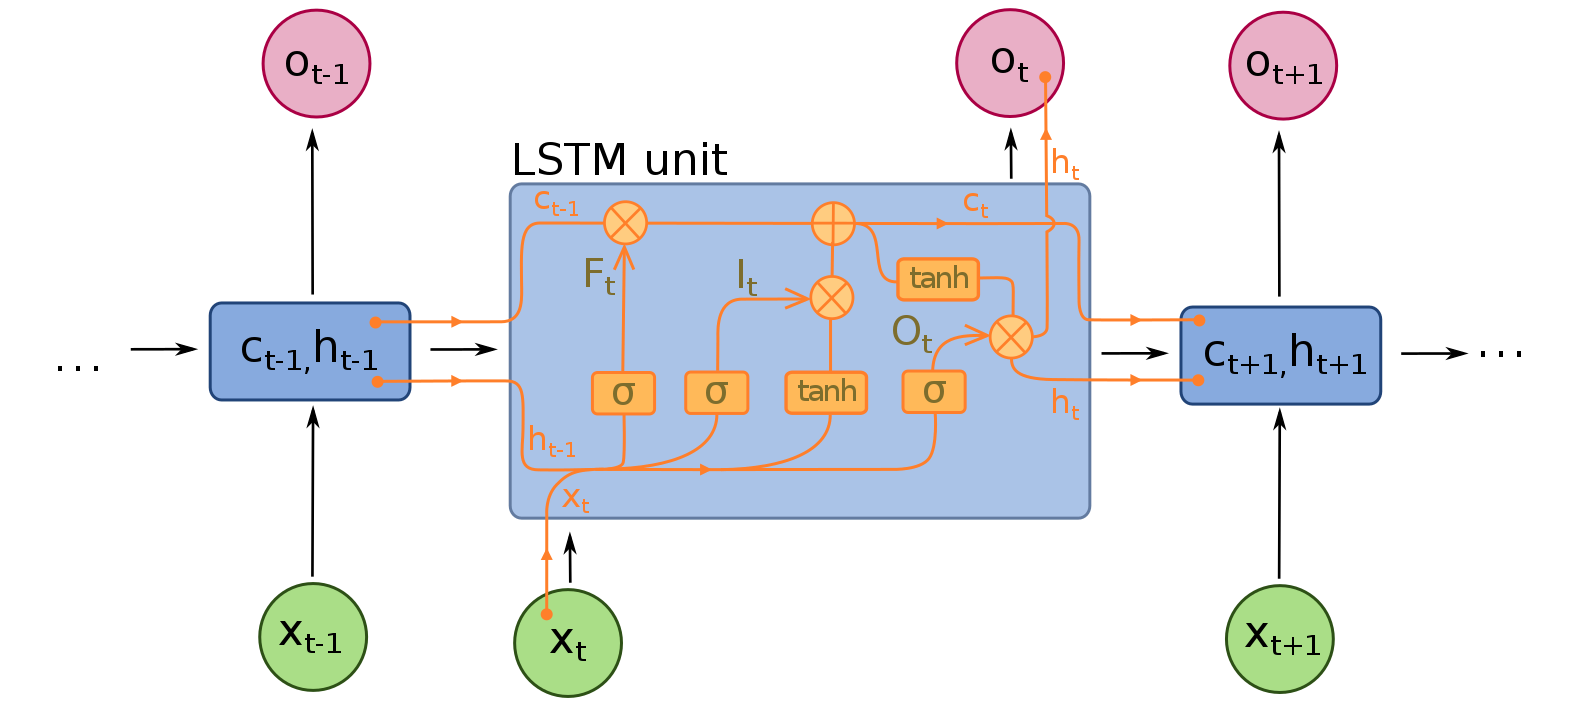
\includegraphics[width=12.5cm]{images/Long_Short-Term_Memory.png}
\end{figure}

Recurrent neural networks (RNNs) are a class of artificial neural network where connections between units form a directed graph along a sequence. In other words, RNNs retain state at one time to the next, using the previous state's output for the current estimate. This characteristic enables multi-stepped time series forecasting. A particular architecture of RNNs known as Long Short-Term Memory (LSTM) allows the model to recognize and retain short-term patterns for long periods of time. This architecture is used best where data from an earlier state needs to be recalled at a later state. Examples of LSTM networks in industry include Google Voice \cite{beaufays}.

\subsection{Motivation}
Senior management needs to interact with this tool.

\subsection{Goal}
The goal is to make the model interactive while tuning and testing.

\section{Object-Oriented Abstraction}
  \begin{itemize}
    \item{Working model in a jupyter notebook}
    \item{Needed to automate runs}
    \item{Needed to organize the code}
    \item{Needed to pass in arbitrary data}
  \end{itemize}

\subsection{Decomposition}
  \begin{itemize}
    \item{Break complex system into parts that are easier to conceive, understand, program, and maintain.}
  \end{itemize}
\subsection{Encapsulation}
  \begin{itemize}
    \item{Restricting components of model}
    \item{Allowing specification of options}
  \end{itemize}

\section{Hyperparameter Optimization}
\begin{itemize}
  \item{Learning paramters (hyperparameters) vs. model parameters (learned parameters or the weights for features in regression)}
  \item{Runtime and compute resources}
\end{itemize}

\subsection{Cross-validation}
Train/test split time series data samples observed at fixed time intervals, in train/test sets.
No shuffling. Successive splits must have higher test indices.
In the kth split, it returns first k folds as train set and the (k+1)th fold as test set.
Note that unlike standard cross-validation methods, successive training sets are supersets of those that come before them.
\subsection{Grid Search}
This search exhaustively generates candidates from a grid of parameter values specified with the \texttt{param\_grid} parameter
\subsection{Results}
\subsection{Discussion}

\section{Systems Engineering}
\subsection{Server Infrastructure}
\subsection{Distributed Task Queue}
Job scheduling via Celery
\subsection{Forecast Visualization}
\subsection{Documentation}

\section{Next Steps}
\subsection{Data Pipeline Automation (Apache Hadoop)}
\subsection{Dimensionality Reduction by Feature Selection}
\subsection{Improving Hyperparameter Optimization Efficiency}
\subsection{Statistical Significance Boundary Visualization}
\subsection{Distributed Machine Learning Clusters}

\section{Conclusion}

\begin{thebibliography}{9}
  % An Empirical Comparison of Machine Learning Models for Time Series Forecasting
  % https://www.tandfonline.com/doi/abs/10.1080/07474938.2010.481556

  % Time series forecasting using a hybrid ARIMA and neural network model
  % https://www.sciencedirect.com/science/article/pii/S0925231201007020

  % Comparison of ARIMA and Artificial Neural Networks Models for Stock Price Prediction
  % https://www.hindawi.com/journals/jam/2014/614342/

  % Hyperparameter optimization - Wikipedia
  % https://en.wikipedia.org/wiki/Hyperparameter_optimization

  % Bayesian information criterion - Wikipedia
  % https://en.wikipedia.org/wiki/Bayesian_information_criterion

  % Building Intelligent Systems: A Guide to Machine Learning Engineering
  % https://books.google.com/books?id=s91PDwAAQBAJ

  % Scaling up Machine Learning
  % https://books.google.com/books?id=9u0gAwAAQBAJ

  % Hidden Technical Debt in Machine Learning Systems
  % https://papers.nips.cc/paper/5656-hidden-technical-debt-in-machine-learning-systems.pdf

  % Diagram of a one-unit Long Short-Term Memory (LSTM) network
  % https://commons.wikimedia.org/w/index.php?curid=60149410

  \bibitem{beaufays}
  Beaufays. (2015, August 11). The neural networks behind Google Voice transcription [Blog post]. Retrieved from https://research.googleblog.com/2015/08/the-neural-networks-behind-google-voice.html.

  % Google voice search: faster and more accurate
  % https://research.googleblog.com/2015/09/google-voice-search-faster-and-more.html
\end{thebibliography}

\end{document}
